% ============================ Enrico Ribiani 16-03-2021 ====================================================================
% Base per i documenti  
\documentclass[12pt]{article}
% ------------ pacchetti necessari ----------------
\usepackage[a4paper, total={6in, 8in},margin=1in]{geometry} % formattazione decente della pagina
\usepackage{graphicx}                            % need for figure
\usepackage{amsmath}
\usepackage{amsfonts}                            % if you want the fonts
\usepackage{amssymb}                             % if you want extra symbols
\usepackage{graphicx}  
\renewcommand{\figurename}{Figura}  
\renewcommand{\contentsname}{Indice}                        % need for figures
\usepackage{mathptmx}
\usepackage{float}                               % serve per mettere tabelle e immagini dove si vuole 
\usepackage[utf8]{inputenc}
\usepackage{textcomp}
\usepackage[hang,flushmargin,bottom]{footmisc}   % footnote format
\usepackage{fancyhdr, lastpage}
\usepackage{titlesec}
\usepackage[table,dvipsnames]{xcolor}
%\pagestyle{fancy}
%\renewcommand{\headrulewidth}{0pt}
%\renewcommand*\contentsname{Indice}
\titleformat{\section}{\normalsize\bfseries}{\thesection.}{1em}{}	% required for heading numbering style
\titleformat*{\section}{\Large\bfseries}
\titleformat*{\subsection}{\large\bfseries}
%\usepackage{siunitx}
%\usepackage{tikz}
\usepackage{circuitikz}
\newcommand{\esourcetowattmeter}[1]{
    \draw (#1)node{W};
    \draw (#1.north) node[circle,draw,anchor=south,inner sep=0,fill=white,minimum width=2.5mm]{\tiny +};
    \draw (#1.south) node[circle,draw,anchor=north,inner sep=0,fill=white,minimum width=2.5mm]{\tiny +};
    \draw (#1.east) node[circle,draw,anchor=west,inner sep=0,fill=white,minimum width=2.5mm]{\tiny -};
    \draw (#1.west) node[circle,draw,anchor=east,inner sep=0,fill=white,minimum width=2.5mm]{\tiny -};
}
%\usepackage[siunitx]{circuitikz}
\usepackage{multirow}
\usepackage{tikz}
\usepackage{amsmath}
\usetikzlibrary{angles,quotes}
\usepackage{placeins}
\usepackage{multirow}
%===================links=================
\usepackage{hyperref}
\hypersetup{
    colorlinks=true,
    linkcolor=Sepia,
    filecolor=Green,      
    urlcolor=Cyan,
    pdftitle={SAMPLE},
    pdfpagemode=FullScreen,
    }
    \usepackage{kvoptions}
    \usepackage{xcolor-material}
    \definecolor{nred}{RGB}{191, 97, 106}
    \definecolor{norange}{RGB}{208, 135, 112}
    \definecolor{nyellow}{RGB}{163, 190, 140}
    \definecolor{ngreen}{RGB}{35, 203, 139}
    \usepackage{colortbl}
    \usepackage{nicematrix}
%===================inizio pagina del titolo=================
\begin{document}
    \begin{titlepage}
    \begin{center}
% ------------------ inizio immagine logo ----------
\begin{figure}
    \centering
    
\includegraphics{~/varie/logo.png}
    \label{fig:logo}
\end{figure}
% ------------------ fine immagine logo ----------
% ------------------ fine immagine logo ----------
-------------------------------------------------------------------------------------\\
\vspace{2\baselineskip}
\large Enrico Ribiani\\
\large 4AUB\\
\vfill

\Huge{\textbf{Esperienza laboratoriale misura delle potenze di un circuito RL}}\\
\vfill

\LARGE{esperienza n°3}\\
\vfill
\large{2-11-2021}
\end{center}
%=============== fine pagina titolo ===============
\end{titlepage}
\tableofcontents

\section{Scopo:}
Misurare le potenze in un circuito RL calcolando poi la potenza assorbita per ottenere il valore della potenza effettiva
e comparare i valori ottenuti con i valori teorici.
\subsection{Materiale}
\begin{itemize}
    \item Resistore da $100\Omega$
    \item Induttore da 0,3 H
    \item Regolatore di tensione 120 V 50 Hz
    \item cavi di collegamento
\end{itemize}
    \subsection{Strumenti}
    \begin{itemize}
        \item Wattmetro
        \item Amperometro
        \item Multimetro che fungerà da voltmetro
    \end{itemize}
\vfill
    \subsection{Schema}
    \begin{figure}[!h]
        \centering
        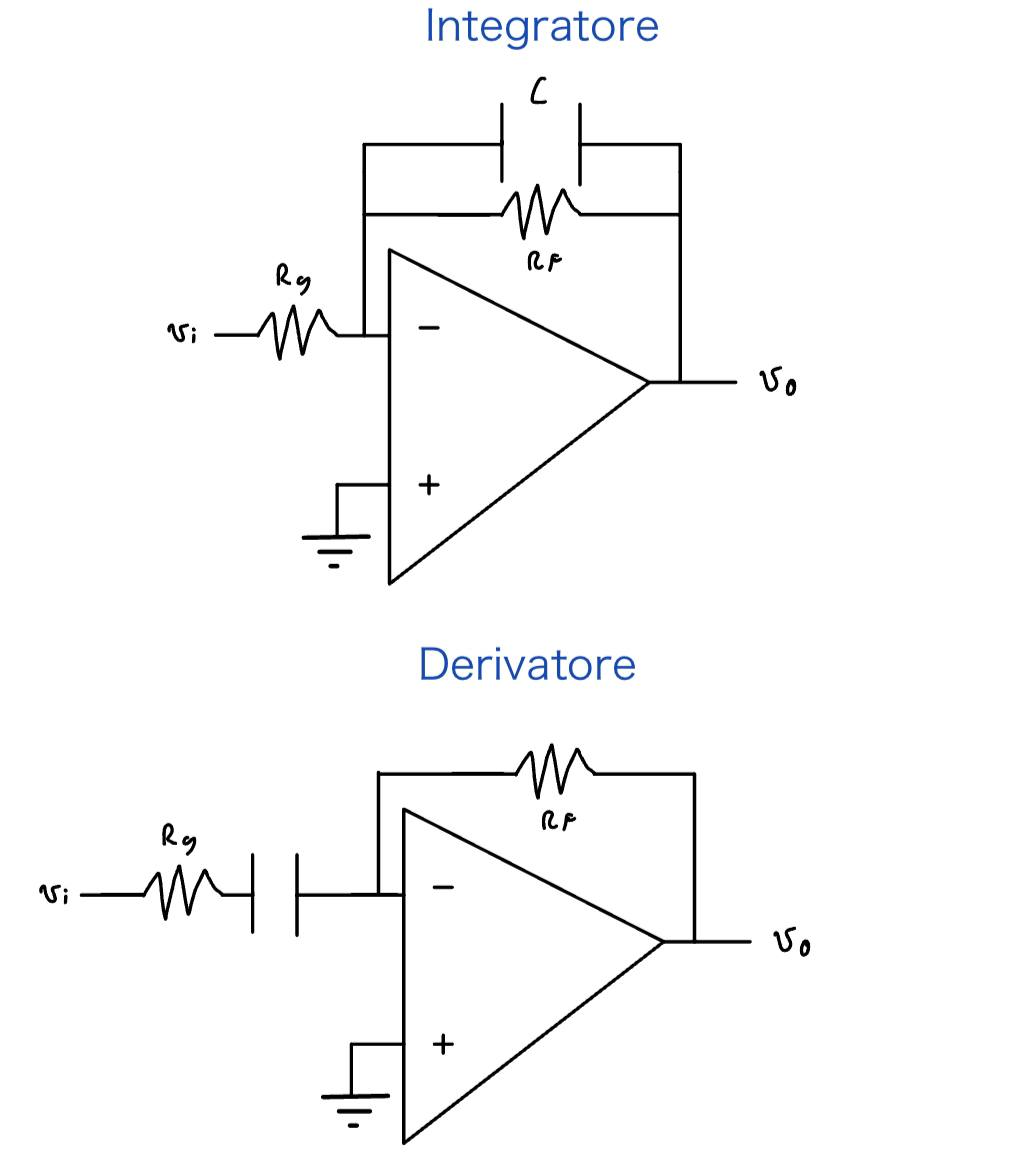
\includegraphics[scale=0.3]{/home/rib/Documenti/latec/potenze-rl/media/schema.jpg}
    \end{figure}
    \FloatBarrier
    
\section{Cenni teorici}
Per effettuare le misure di potenza abbiamo bisogno di uno strumento speciale, chiamato \textit{Wattmetro}, questo strumento misura
la potenza attiva basandosi sul metodo volt-amperometrico, infatti questo strumento è l'insieme di un volltmentro e di un amperometro, e ha 
4 morsetti ossia due coppie, una per l'amperometro e due per il voltmetro.\\
Per avere tutte le poteze di un circuito abbiamo bisogno anche di un voltmetro e un amperometro separati dal wattmetro che oltre a indicarci se 
rischiamo di bruciare il wattmetro uscendo dai valori massimi sopportati ci consentono anche di ricavare la potenza apparente o S tramite $V \cdot I$.\\
Avendo la potenza apparente e quella attiva si può senza problema ricavare la potenza reattiva Q.

\section{Procedimento/Analisi}
Per prima cosa si controlla che il regolatore di tensione non sia collegato alla rete elettrica, dopodiché si procede a montare il 
circuito ossia collegare tutti i componenti e gli strumenti con gli appositi cavi.\\
Si decide se iniziare a collegare la parte di corrente (amperometro) o di tensione (voltmetro) utilizzand due colori diversi per i cavi che collegheranno le due parti.\\
Si consiglia di andare a posizionare e collegare tutti i componenti nell'ordine in cui sono disegnati sullo schema, ma lasciando il wattmetro come ultima cosa da 
collegare in quanto con i suoi 4 morsetti è il più complesso.\\
Dopo aver collegato tutti i componenti ci si assicura che il trasformatore di tensione sia a 0 e si collega alla rete elettrica, successivamente
si va ad aumentare la tensione lentamente osservando tutti e tre gli strumenti per osservare eventuali enomalie fino a raggiungere la tensione di 120V.\\
Una volta raggiunta la tensione desiderata si prendono le misure richieste in tabella e si annota la resistenza interna del wattmetro alla tensione da noi 
utilizzata.\\ 


    \subsection{Tabelle}
\begin{center}
    
    \begin{table}[!h]
       \centering
        \begin{tabular}{|p{2cm}|p{3cm}|p{2cm}|p{2cm}|p{2cm}|p{3cm}|}
        \hline
        \rowcolor{BrickRed} \multicolumn{5}{c}{Amperometro}\\
        \hline
        \rowcolor{BrickRed!70} FS[A] & K=$\frac{FS}{ND}$ [ma] & ND lette & i[ma] & Ea=$\frac{FS}{ND}\cdot CL$\\
        \hline
        \rowcolor{BrickRed!50} 1,2 & 10 & 89 & 890 & 0,005 \\
        \hline
    \end{tabular}
    
\vspace{1 cm}
\begin{tabular}{cc}
    
    \begin{tabular}[t]{|c|}
        \hline
        \rowcolor{LimeGreen} Voltmetro\\
        \hline
        \rowcolor{LimeGreen!70} V[V]\\
        \hline
        \rowcolor{LimeGreen!50} 120,38\\
        \hline
    \end{tabular}&

    \begin{tabular}[t]{|c|c|}
        \hline
        \rowcolor{Blue!80} CL & 0,5 \\
        \hline
        \rowcolor{Aquamarine!90} Rsper & $98,7 \Omega$\\
        \hline
        \rowcolor{SeaGreen!90} Rwattmetro & $40k\Omega$\\
        \hline
    \end{tabular}
    \vspace{1 cm}
\end{tabular}

    \begin{tabular}{|c|c|c|c|c|c|}
        \hline
        \rowcolor{BurntOrange} \multicolumn{6}{c}{Wattmetro}\\
        \hline
        \rowcolor{BurntOrange!70} Fs & K & ND lette & Pm[W] & Pa[W] & Pz[W]\\
        \hline
    \rowcolor{BurntOrange!50} 120 & 1 & 68 & 68 & 0,36 & 67,63 \\
        \hline
    \end{tabular}


\end{table}
\vspace{1 cm}
CL = classe dello strumento data da $\epsilon_a \cdot K$\\
$\epsilon_a=\frac{Fondoscala}{n° divisioni} \cdot CL$
\end{center}
    \subsection{Calcoli}
    \begin{center}
        \textbf{Calcoli teorici}\\
        \vspace{0.5 cm}
        $X_L = 2\pi \cdot f \cdot L = 2\pi \cdot 50 Hz \cdot 0,3 H= 94,2 \Omega$\\
        $Z=\sqrt{R^2 + {X_L}^2}=137,4 \Omega$\\
        $\vec{Z}=(R+jX_L)=(100+j92,2)\Omega$\\
        $I=\frac{V}{Z}=\frac{120 V}{137,4 \Omega}=0,87 A$\\
    \vspace{0.5 cm}
        $\varphi=\arctan(\frac{X_L}{R})=43,3$°\\
    \vspace{0.5 cm}
        \colorbox{RedOrange}{P}$=R\cdot I^2= 100 \cdot 0,87^2=75,7W$\\
        \colorbox{Dandelion}{Q}$=X_L \cdot  I^2=94,2 \cdot 0,87^2= 71,3 VAR $\\
        \colorbox{Goldenrod}{S}$=Z \cdot I^2= 137,4 \Omega \cdot 0,87^2=104 VA$\\
    \vspace{1 cm}
        \textbf{Calcoli sperimentali}\\
       \colorbox{Orange}{$P_{assorbita}$} $=\frac{V^2}{Ramp}=0,36 W$\\
       \colorbox{Peach}{$P_z$} $=P_m - P_a=68-0,36=67,6[W]$\\
       \vspace{10 mm}
       \colorbox{TealBlue}{S} $=V\cdot I=120,4V \cdot 0,89 A =107,2 [VA]$\\
       
        
       \colorbox{Blue!76}{Q} $=\sqrt{S^2 - P^2}=\sqrt{107,2^2 - 67,6^2}=83 [W] $\\% (Utilizzando i valore della potenza reattiva misurato con il wattmetro.)
    \end{center}
\section{Conclusioni}
A parte qualche piccola discrepanza inevitabile i valori sperimentali che non riguardano il wattmetro sono accettabili mentre la potenza attiva
P misurata con il wattmetro presenta circa un 10\% di discrepanza non giustificato dall'errore assoluto o dall'assorbimento.\\
È probabile che questa discrepanza eccessiva sia dovuta dalla somma di tutte gli errori dati dagli strumenti di misura resi più evidenti dal fatto che 
il wattmetro sia formato da un amperometro e un voltmetro uniti.
\end{document}
